\documentclass[addpoints]{exam}

\printanswers
\CorrectChoiceEmphasis{\color{red}\bfseries}
\usepackage{amssymb, amsmath, amsfonts}
\usepackage{geometry}
\usepackage{graphicx}
\usepackage{tikz}
\usetikzlibrary{calc}
\usepackage{pgfplots}
\usepackage{multirow,array} % for payoff matrix formatting
\usepackage[colorlinks,pdfusetitle,urlcolor=blue,citecolor=blue,linkcolor=blue]{hyperref}
\usepackage{bbding} % dingbats fonts

\usepackage{adjustbox}

\definecolor{crimson}{RGB}{ 170, 4, 36 }
\definecolor{darkblue}{RGB}{ 4, 47, 170 }
\definecolor{brown}{RGB}{ 111, 71, 2 }
\definecolor{periwinkle}{RGB}{ 90, 177, 204 }
\definecolor{ducksgreen}{HTML}{007030}

\geometry{left=1.0in,right=1.0in,top=1.0in,bottom=1.0in}
\pagestyle{headandfoot}
\lhead{EC327 Game Theory}
\chead{Homework 5}
\rhead{Fall 2025}
\runningheadrule

\title{
    \textbf{Econ 327: Game Theory} \\ 
    Homework $\#5$
    }
\author{University of Oregon}
\date{Due: Nov. 7$^{th}$}

% exam-type question formatting
\renewcommand{\thequestion}{\textbf{Q\arabic{question}}}
\bracketedpoints

\begin{document}

\maketitle

\begin{center}
  \gradetable[h][questions]
\end{center}

\vspace{0.5in}

\begin{center}
  \textbf{For homework assignments:}
\end{center}

\begin{itemize}

%  \item DO NOT write your name:
%  this assignment will be graded anonymously. 
%  If you want to, you can include your student ID instead.

  \item Complete \textit{all} questions and parts.

  % I will select one question at random to be graded
  % according to the rubric on Canvas.

  \item You will be graded on not only the content of your work
    but on how clearly you present your ideas.
    Make sure that your handwriting is legible.
    Please use extra pages if you run out of space 
    but make sure that all parts of a question 
    are in the correct order when you submit.

  \item You may choose to work with others,
  but everyone must submit to Canvas individually.

  Please include the names of everyone who you worked with 
  below your own name.
 
\end{itemize}

\vspace{1.0in}

\makebox[.6\textwidth]{Name\enspace\hrulefill}

\vspace{0.5in}

% \begin{center}
%   \fbox{\fbox{\parbox{5.5in}{\centering
%     Answer the questions in the spaces provided on the
%     question sheets. If you run out of room for an answer,
%     continue on the back of the page or another sheet of paper.}}}
% \end{center}

\newpage

\begin{questions}

\question

Follow the steps for the game below:
  \begin{center}
      \begin{tabular}{*{4}{c|}}
        \multicolumn{2}{c}{} & \multicolumn{2}{c}{$P_2$} \\ \cline{3-4}
        \multicolumn{1}{c}{} & & $B$ & $D$ \\ \cline{2-4}
        \multirow{2}*{$P_1$}
        & $J$ & 6,6 &  4, 0 \\ \cline{2-4}
        & $K$ & 0,3 & 10,15 \\ \cline{2-4}
      \end{tabular}
    \end{center}
  
  \begin{parts}
  \part[4] 

  Define mixed strategies for each player.
  Make sure to define all variables you introduce.

  \begin{solution}
    
    Let $\alpha$ be the probability that $P_1$ plays $J$.

    Player 1's mixed strategy will be $\mathbf{(\alpha J, (1-\alpha) K)}$ 
    (and zero weight on $H$ and $L$).

    Let $\beta$ be the probability that $P_2$ plays $B$.

    Player 2's mixed strategy will be $\mathbf{(\beta B, (1-\beta) D)}$
    (and zero weight on $A$ and $C$). 

    \par\noindent\rule{\textwidth}{0.4pt}

    The notation doesn't have to match, 
    but a correct answer will have one probability associated with each player
    and the remaining probability on the proper player's other strategy played in equilibrium.

  \end{solution}

  \part[4]
  Graph Player 1's expected utilities as functions of
  Player 2's mixed strategy you defined in part (a).

  \part[4]
  Graph Player 2's expected utilities as functions of
  Player 1's mixed strategy you defined in part (a).
  \begin{solution}

    \begin{minipage}{.5\textwidth}
      (b) \\
      \centering
       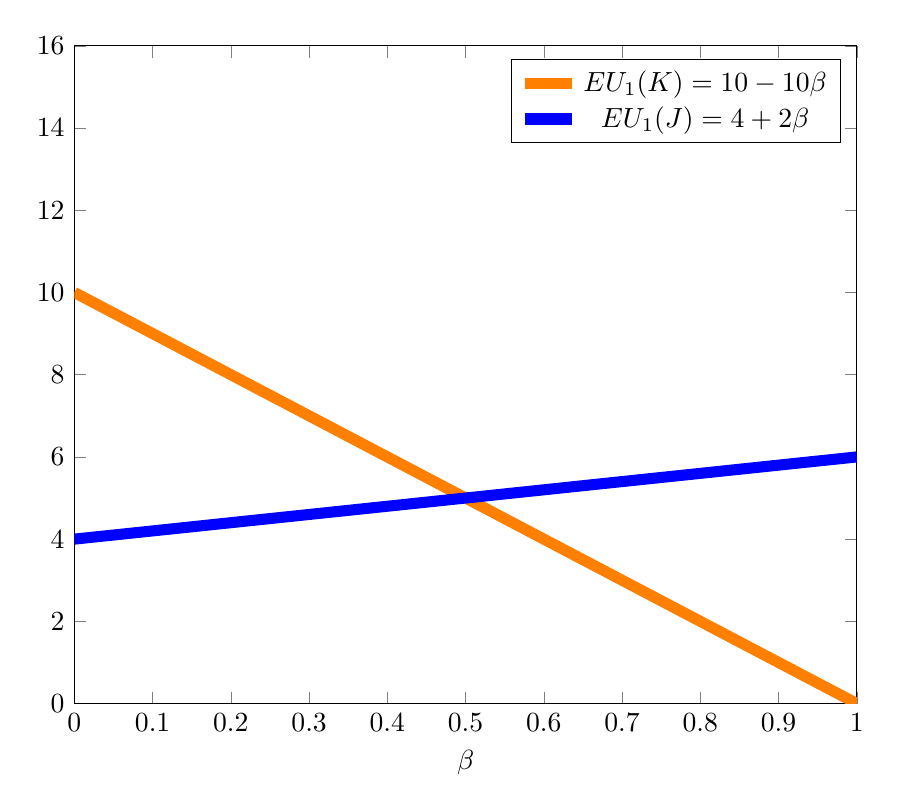
\begin{tikzpicture}
         \begin{axis}[
           width=.95\textwidth,
           xlabel={$\beta$},
           % ylabel={Player 2's Expected Utility}
           xmin=0, xmax=1,
           ymin=0, ymax=16,
           ]
           % EU(K)
           \addplot [
             line width=4pt,
             domain=0:1,
             samples=10,
             color=orange,
           ]
           {10 - 10*x};
           \addlegendentry{\(EU_1(K)=10-10\beta\)}
           % EU(J)
           \addplot [
             line width=4pt,
             domain=0:1,
             samples=10,
             color=blue,
           ]
           {4 + 2*x};
           \addlegendentry{\(EU_1(J)=4+2\beta\)}

         \end{axis} 
       \end{tikzpicture}
    \end{minipage}
    \begin{minipage}{.5\textwidth}
      (c) \\
      \centering
       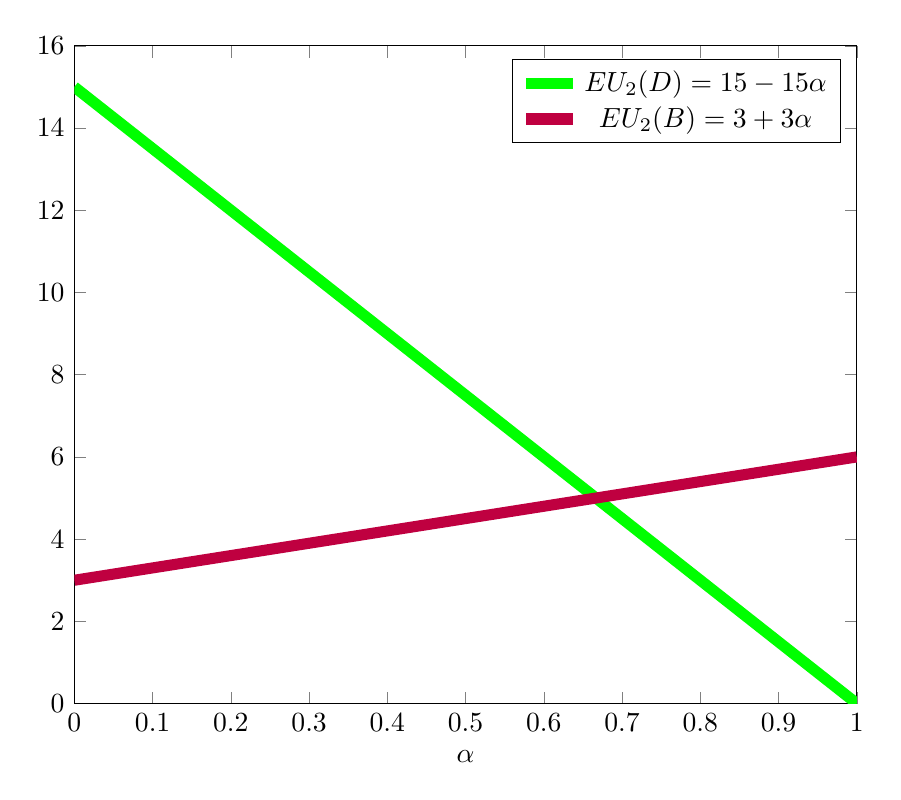
\begin{tikzpicture}
         \begin{axis}[
           width=.95\textwidth,
           xlabel={$\alpha$},
           % ylabel={Player 2's Expected Utility}
           xmin=0, xmax=1,
           ymin=0, ymax=16,
           ]
           % EU(D)
           \addplot [
             line width=4pt,
             domain=0:1,
             samples=10,
             color=green,
           ]
           {15 - 15*x};
           \addlegendentry{\(EU_2(D)=15-15\alpha\)}
           % EU(B)
           \addplot [
             line width=4pt,
             domain=0:1,
             samples=10,
             color=purple,
           ]
           {3 + 3*x};
           \addlegendentry{\(EU_2(B)=3+3\alpha\)}

         \end{axis} 
       \end{tikzpicture}
    \end{minipage}


  \end{solution}

  \part[4]
  Solve for all Nash equilibria in this game
  (mixed and pure strategies).
  A complete answer will include all calculations used 
  and a graph of best response functions.

  \begin{solution}

    When will Player 1 be indifferent between $J$ and $K$:
    \begin{tabular}{r c l}
      $EU_1(J)$ & = & $EU_1(K)$ \\ 
      $6\beta + 4 (1-\beta)$ & = & $0\beta + 10(1-\beta)$ \\
      $4 + 2\beta$ & = & $10 - 10\beta$ \\ 
      $\beta$ & = & $1/2$ \\ 
    \end{tabular}

    When will Player 2 be indifferent between $B$ and $D$:
    \begin{tabular}{r c l}
      $EU_2(B)$ & = & $EU_2(D)$ \\ 
      $6\alpha + 3 (1-\alpha)$ & = & $0\alpha + 15(1-\alpha)$ \\
      $3 + 3\alpha$ & = & $15 - 15\alpha$ \\ 
      $\alpha$ & = & $2/3$ \\ 
    \end{tabular}

    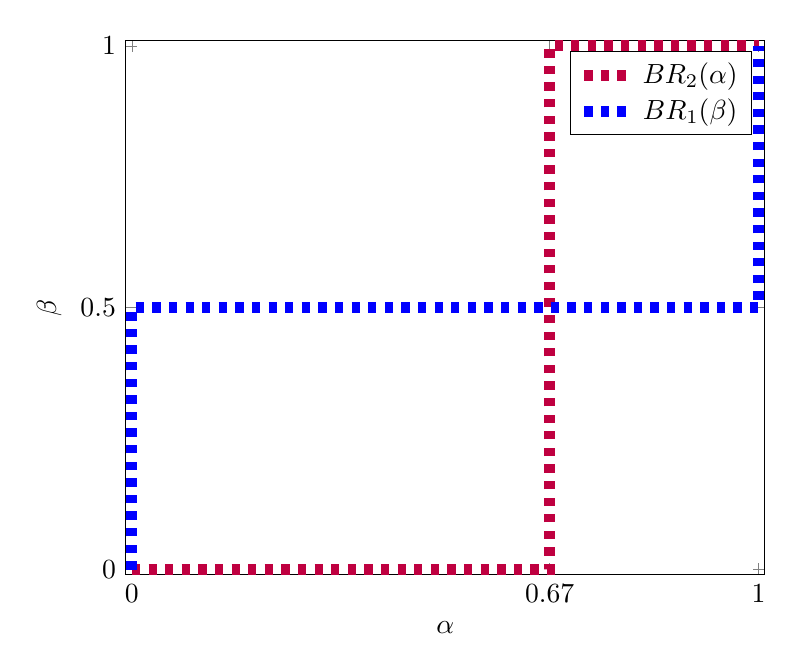
\begin{tikzpicture}
      \begin{axis}[
        width=.8\textwidth,
        xlabel={$\alpha$},
        ylabel={$\beta$},
        xmin=-0.01, xmax=1.01,
        ymin=-0.01, ymax=1.01,
        xtick={0,2/3,1},
        ytick={0,1/2,1},
        ]
        \addplot [
        dashed,
        line width=4pt,
        const plot,
        color=purple
        ] coordinates {
        (0,0)
        (2/3,0)
        (2/3,1)
        (1,1)
        };
        \addlegendentry{\(BR_2(\alpha)\)}
        \addplot [
        dashed,
        line width=4pt,
        const plot,
        color=blue,
        ] coordinates {
        (0,0)
        (0,1/2)
        (1,1/2)
        (1,1)
        };
        \addlegendentry{\(BR_1(\beta)\)}
      \end{axis}
    \end{tikzpicture}

    \begin{itemize}
      \item 
      \textbf{MSNE:} $\{\sigma_1 = (2/3 J, 1/3 K), \sigma_2 = (1/2 B, 1/2 D)\}$
      \item \textbf{PSNE:}
      \begin{itemize}
        \item $\{\sigma_1 = K, \sigma_2 = D\}$
        \item $\{\sigma_1 = J, \sigma_2 = B\}$
      \end{itemize}
    \end{itemize}

  \end{solution}
\end{parts}

\newpage

\question

Consider the strategic form game below: 

\begin{table}[!h]
  \begin{center}
    \begin{tabular}{*{5}{c|}}
      \multicolumn{2}{c}{} & \multicolumn{3}{c}{$P_2$} \\ \cline{3-5}
      \multicolumn{1}{c}{} &  & \textbf{Left} & \textbf{Center} & \textbf{Right} \\ \cline{2-5} 
      \multirow{4}*{$P_1$}
      & \textbf{Top}    & 3 , 1 & 3 , 2 & 0 , 2 \\ \cline{2-5}
      & \textbf{Middle} & 1 , 2 & 2 , 1 & 1 , 2 \\ \cline{2-5}
      & \textbf{Bottom} & 0 , 2 & 3 , 2 & 3 , 1 \\ \cline{2-5} 
    \end{tabular}
  \end{center}
\end{table}

\begin{parts}
  \part[4]
  Find any \textbf{pure strategy} Nash equilibria
  \begin{solution}
    (Top, Center) and (Bottom, Center) are the pure-strategy Nash
  \end{solution}
  \part[4]
  Consider the following mixed strategy profile: 
  \begin{itemize}
    \item Player 1 plays 1/3 \textbf{Top}, 1/3 \textbf{Middle}, and 1/3 \textbf{Bottom}
    \item Player 2 plays 1/3 \textbf{Left}, 1/3 \textbf{Center}, 1/3 \textbf{Right}
  \end{itemize}
  Check whether this is a \textbf{mixed strategy Nash equilibrium} and explain why or why not. 
  \begin{solution}
    \begin{align*}
      EU_1(\text{Top}) & = 3(1/3) + 3(1/3) + 0(1/3) = 2 \\
      EU_1(\text{Middle}) & = 1(1/3) + 2(1/3) + 1(1/3) = \frac{4}{3} \\
      EU_1(\text{Bottom}) & = 0(1/3) + 3(1/3) + 3(1/3) = 2 \\
    \end{align*}
    So Player 1 would unilaterally deviate to playing less of Middle
    which has a strictly lower payoff than Top or Bottom,
    conditional on Player 2 playing (1/3, 1/3, 1/3). \XSolidBrush \\
    \textbf{Not an MSNE}
  \end{solution}
  \part[4]
  Now consider the strategy profile:
  \begin{itemize}
    \item Player 1 plays 1/3 \textbf{Top}, 1/3 \textbf{Middle}, and 1/3 \textbf{Bottom}
    \item Player 2 plays 1/2 \textbf{Left}, 0 \textbf{Center}, 1/2 \textbf{Right}
  \end{itemize}
  Check whether this is a \textbf{mixed strategy Nash equilibrium} and explain why or why not.
  \begin{solution}
    \begin{align*}
      EU_1(\text{Top}) & = 3(1/2) + 3(0) + 0(1/2) = \frac{3}{2} \\
      EU_1(\text{Middle}) & = 1(1/2) + 2(0) + 1(1/2) = 1 \\
      EU_1(\text{Bottom}) & = 0(1/2) + 3(0) + 3(1/2) = \frac{3}{2} \\
    \end{align*}
    So Player 1 would unilaterally deviate to playing less of Middle
    which has a strictly lower payoff than Top or Bottom,
    conditional on Player 2 playing (1/2, 0, 1/2). \XSolidBrush \\
    \textbf{Not an MSNE}
  \end{solution}
  \part
  Now consider the strategy profile:
  \begin{itemize}
    \item Player 1 plays 1/4 \textbf{Top}, 0 \textbf{Middle}, and 3/4 \textbf{Bottom}
    \item Player 2 plays 0 \textbf{Left}, 1 \textbf{Center}, 0 \textbf{Right}
  \end{itemize}
  Check whether this is a \textbf{mixed strategy Nash equilibrium} and explain why or why not.
  \begin{solution}
    \begin{align*}
      EU_1(\text{Top}) & = 3(0) + 3(1) + 0(0) = 3 \\
      EU_1(\text{Middle}) & = 1(0) + 2(1) + 1(0) = 2 \\
      EU_1(\text{Bottom}) & = 0(0) + 3(1) + 3(0) = 3 \\
    \end{align*}
    So Player 1 is indifferent between Top and Bottom,
    and will never play Middle.
    This is consistent w/ them playing (1/4, 0, 3/4) mixed-strategy $\checkmark$. \\
    \begin{align*}
      EU_2(\text{Left}) & = 1(1/4) + 2(0) + 2(3/4) = \frac{7}{4} \\
      EU_2(\text{Center}) & = 2(1/4) + 1(0) + 2(3/4) = 2 \\
      EU_2(\text{Right}) & = 2(1/4) + 2(0) + 1(3/4) = \frac{5}{4} \\
    \end{align*}
    So Player 2's strictly dominat strategy is only Center $\checkmark$. \\
    \textbf{\{(1/4, 0, 3/4), Center\} is an MSNE}
  \end{solution}
\end{parts}

\newpage

\question
Consider the following game:\footnote{Dixit, Skeath, \& McAdams, \textit{Games of Strategy}, 4th Edition}
  \begin{table}[h!]
    \centering
    \setlength{\extrarowheight}{2pt}
    \begin{tabular}{*{4}{c|}}
      \multicolumn{2}{c}{} & \multicolumn{2}{c}{Colin} \\\cline{3-4}
      \multicolumn{1}{c}{} &       & Yes & No   \\\cline{2-4}
      \multirow{3}*{Rowena}  & Yes & $x$,$x$ & 0,1 \\\cline{2-4}
                             & No  & 1,0 & 1,1 \\\cline{2-4}
    \end{tabular}
  \end{table}
  \begin{parts}
    \part[4]
    For what values of $x$ does this game have a unique Nash equilibrium?
    What is that equilibrium?
    \begin{solution}
      If $x<1$, then \texttt{No} is a dominant strategy
      and (\texttt{No, No)} is the unique Nash.
    \end{solution}
    \part[4]
    For what values of $x$ does this game have a mixed strategy equilibrium?
    With what probability, expressed in terms of $x$
    does each player play Yes in this mixed-strategy equilibrium?
    \begin{solution}
      For there to be an MSNE, a player must be indifferent between pure strategies.
      This is a symmetric game.
      Either player is indifferent between \texttt{Yes} and \texttt{No}
      if:
      \[px + 0(1-p) = 1\]
      where $p$ is the probability the \textit{other player} chooses \texttt{Yes}. \\
      For $p$ to be a meaningful probability, $0\leq \frac{1}{x} \leq 1$,
      or \underline{$x\geq 1$}.
    \end{solution}
    \part[4]
    Let $x=3$. Graph the best-response curves of Rowena and Colin
    against each other's mixed strategy probability
    on the same graph.
    Label all Nash equilibria in pure and mixed strategies.
    \begin{solution} \\
    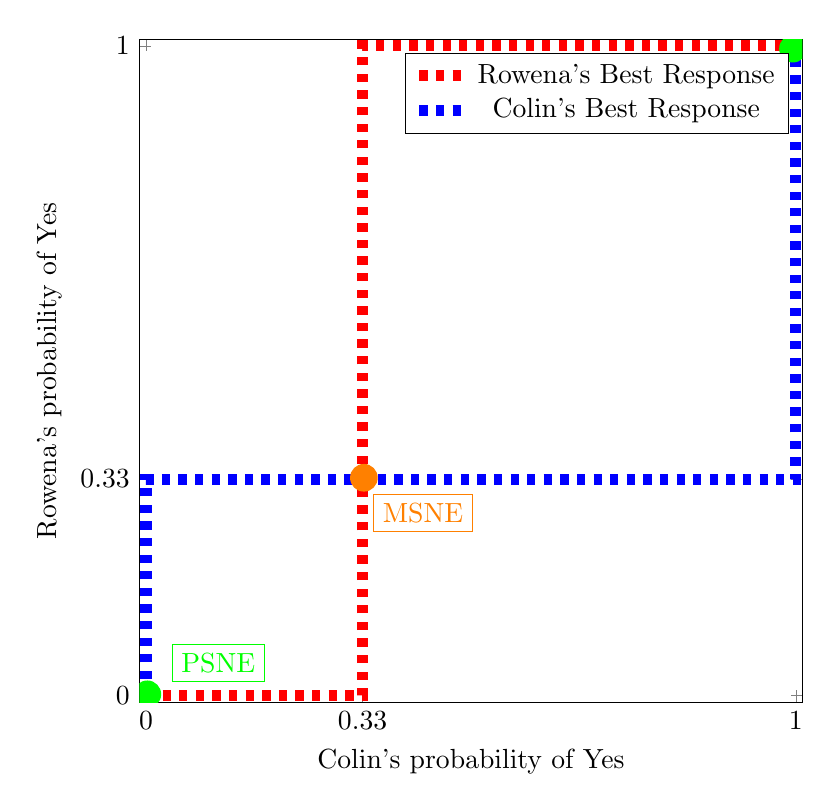
\begin{tikzpicture}
      \begin{axis}[
        width=10cm,
        height=10cm,
        xlabel={Colin's probability of Yes},
        ylabel={Rowena's probability of Yes},
        xmin=-0.01, xmax=1.01,
        ymin=-0.01, ymax=1.01,
        xtick={0,1/3,1},
        ytick={0,1/3,1},
        ]
        \addplot [
        dashed,
        line width=4pt,
        const plot,
        color=red
        ] coordinates {
        (0,0)
        (1/3,0)
        (1/3,1)
        (1,1)
        };
        \addlegendentry{Rowena's Best Response}
        \addplot [
        dashed,
        line width=4pt,
        const plot,
        color=blue,
        ] coordinates {
        (0,0)
        (0,1/3)
        (1,1/3)
        (1,1)
        };
        \addlegendentry{Colin's Best Response}
        \node (B) [draw,orange] at (3.6cm,2.4cm) {MSNE};
        \fill [orange] (2.85cm,2.85cm) circle (5pt);
        \fill [green] (.1cm,.1cm) circle (5pt);
        \fill [green] (8.3cm,8.3cm) circle (5pt);
        \node (A) [draw,green] at (1cm,.5cm) {PSNE};
      \end{axis}
    \end{tikzpicture}

    \end{solution}

    \part[4]
    Let $x=1$. Graph the best-response curves of Rowena and Colin
    against each other's mixed strategy probability
    on the same graph.
    Label all the Nash equilibria in pure and mixed strategies.
    \begin{solution} \\
    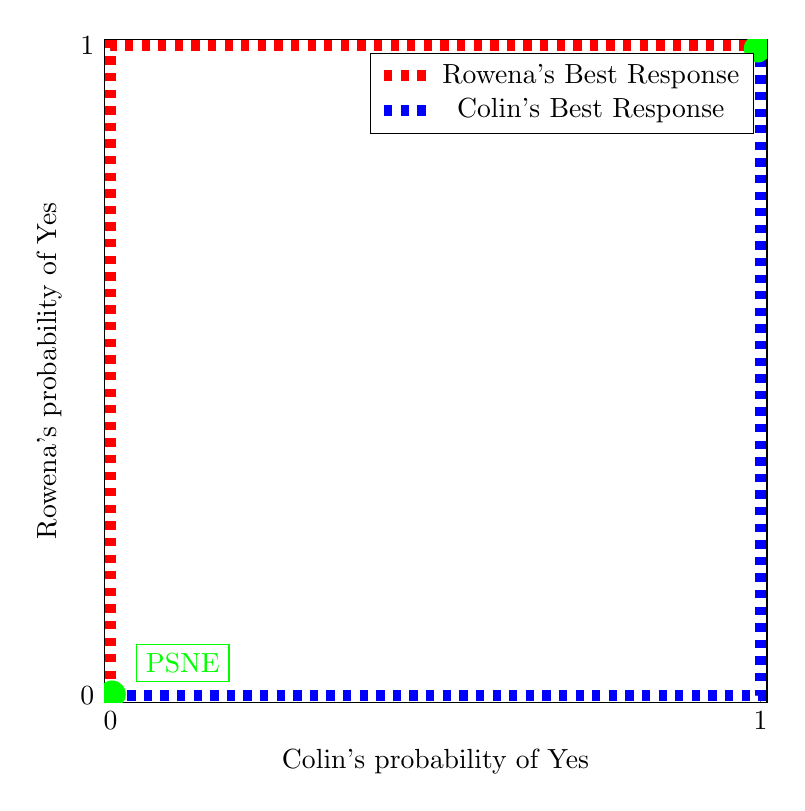
\begin{tikzpicture}
      \begin{axis}[
        width=10cm,
        height=10cm,
        xlabel={Colin's probability of Yes},
        ylabel={Rowena's probability of Yes},
        xmin=-0.01, xmax=1.01,
        ymin=-0.01, ymax=1.01,
        xtick={0,1},
        ytick={0,1},
        ]
        \addplot [
        dashed,
        line width=4pt,
        const plot,
        color=red
        ] coordinates {
        (0,0)
        (0,1)
        (1,1)
        };
        \addlegendentry{Rowena's Best Response}
        \addplot [
        dashed,
        line width=4pt,
        const plot,
        color=blue,
        ] coordinates {
        (0,0)
        (1,0)
        (1,1)
        };
        \addlegendentry{Colin's Best Response}
        \fill [green] (.1cm,.1cm) circle (5pt);
        \fill [green] (8.3cm,8.3cm) circle (5pt);
        \node (A) [draw,green] at (1cm,.5cm) {PSNE};
      \end{axis}
    \end{tikzpicture}
  \end{solution}
  \end{parts}

% \newpage

% \question
% For each of the following game tables, find all mixed-strategy Nash equilibria.
% \begin{parts}
%   \part[4]
%   \begin{table}[h!]
%     \centering
%     \setlength{\extrarowheight}{2pt}
%     \begin{tabular}{*{4}{c|}}
%       \multicolumn{2}{c}{} & \multicolumn{2}{c}{Player 2} \\\cline{3-4}
%       \multicolumn{1}{c}{} &          & Left & Right   \\\cline{2-4}
%       \multirow{3}*{Player 1}  & Up   & 3,3 & 9,4 \\\cline{2-4}
%                                & Down & 5,2 & 6,1 \\\cline{2-4}
%     \end{tabular}
%   \end{table}
%   \part[4]
%   \begin{table}[h!]
%     \centering
%     \setlength{\extrarowheight}{2pt}
%     \begin{tabular}{*{4}{c|}}
%       \multicolumn{2}{c}{} & \multicolumn{2}{c}{Player 2} \\\cline{3-4}
%       \multicolumn{1}{c}{} &       & S   & T   \\\cline{2-4}
%       \multirow{3}*{Player 1}  & F & 7,3 & 2,4 \\\cline{2-4}
%                                & G & 5,2 & 6,1 \\\cline{2-4}
%                                & H & 6,1 & 5,4 \\\cline{2-4}
%     \end{tabular}
%   \end{table}
%   \part[4]
%   \begin{table}[h!]
%     \centering
%     \setlength{\extrarowheight}{2pt}
%     \begin{tabular}{*{4}{c|}}
%       \multicolumn{2}{c}{} & \multicolumn{2}{c}{Player 2} \\\cline{3-4}
%       \multicolumn{1}{c}{} &       & X   & Y \\\cline{2-4}
%       \multirow{3}*{Player 1}  & A & 2,3 & 6,1 \\\cline{2-4}
%                                & B & 4,2 & 1,3 \\\cline{2-4}
%                                & C & 3,1 & 2,4 \\\cline{2-4}
%     \end{tabular}
%   \end{table}
% \end{parts}

% \begin{parts}
%   \part[4]
%   \begin{table}[h!]
%     \centering
%     \setlength{\extrarowheight}{2pt}
%     \begin{tabular}{*{4}{c|}}
%       \multicolumn{2}{c}{} & \multicolumn{2}{c}{Watson} \\\cline{3-4}
%       \multicolumn{1}{c}{} &         & Cliffs & Town \\\cline{2-4}
%       \multirow{3}*{Holmes} & Cliffs & -2,1   & 0,0 \\\cline{2-4}
%                             & Town   & -3,0   & 1,1 \\\cline{2-4}
%     \end{tabular}
%   \end{table}
%   \part[4]
%   \begin{table}[h!]
%     \centering
%     \setlength{\extrarowheight}{2pt}
%     \begin{tabular}{*{4}{c|}}
%       \multicolumn{2}{c}{} & \multicolumn{2}{c}{Van} \\\cline{3-4}
%       \multicolumn{1}{c}{} &         & Duck & Rabbit   \\\cline{2-4}
%       \multirow{3}*{Eddie}  & Duck   & -2,1 & 0,0 \\\cline{2-4}
%                             & Rabbit & 0,0  & 1,-2 \\\cline{2-4}
%     \end{tabular}
%   \end{table}
%   \part[4]
%   \begin{table}[h!]
%     \centering
%     \setlength{\extrarowheight}{2pt}
%     \begin{tabular}{*{4}{c|}}
%       \multicolumn{2}{c}{} & \multicolumn{2}{c}{Player 2} \\\cline{3-4}
%       \multicolumn{1}{c}{} &         & Left & Right   \\\cline{2-4}
%       \multirow{3}*{Player 1} & Up   & 6,9  & 12,8 \\\cline{2-4}
%                               & Down & 9,4  & 7,10 \\\cline{2-4}
%     \end{tabular}
%   \end{table}
% \end{parts}

\end{questions}
\end{document}